\section{Experiment}
\label{sec:experiment}
In this section, the design, realization and the result of experiments will be stated.
Due to the relatively large scale test is needed, experiments are deployed on Google Cloud Platform. 
In addition, the experiments run on \texttt{TensorFlow-GPU 1.12.0} rather than CPU version, which is used during the development.
Consequently the result there may be slightly different.

\subsection{Design}
The aim of the experiments is to explore the capability of the network for understanding the logical feature.
The experiment is designed into two parts.
The first part is designed to test the stability of the training with respect to all the possible graphs with the same scale.
So that the reliability of a single test can be estimated.
The reason to estimate the reliability of a single test is that extensive and complete experiments are not feasible when the graph is big, due to the exponential growth of possible graph pairs.
However, even for relatively small graph, generate all possible cases would be very time-consuming. 
And that is also the reason why generate-all-generator was abandoned (see Section \ref{sec:imptestcasegenerator}).
Instead, sampling is chosen as an alternative plan.
Random test case generator can be seen as a sampling machine.
By generate multiple groups of graphs with different density, the sampling is expected to cover most of the combinations.
Specifically, the experiment parameters will be shown in Listing \ref{lst:wideexp}.


% \captionof{listing}{Wide experiments arguments \label{lst:wideexp}}
% \vspace{-0.5em}
\begin{code}
\caption{Wide experiments arguments}
\label{lst:wideexp}
\begin{minted}[linenos, frame=single,breaklines]{python}
# ========== wide experiments ==========
# ---- ARGUMENTS ----
nodes_num = 5 
edge_type_num = 3 
c_type = random 
case_number = 10000 
graph_density = [0.1, 0.2, 0.3, 0.4, 0.5, 0.6, 0.7, 0.8, 0.9]
p_rate = 0.5 
learning_rate = 0.1
epochs = 500
batch_size = 100
# -------------------

\end{minted}
\end{code}

The second part of the experiments is aiming to find the limit of this network, namely the algorithm designed in this project (see Figure \ref{fig:mlp_model}).
In this part, the algorithm will be trained on graphs with different scale, i.e. bigger graphs.
And by comparison, the limitation of the network can be estimated.
Notice that for graphs with different scale, the network will be slightly different, i.e. only the length of the input layer and re-represent layer (see Figure \ref{fig:mlp_model}) will be different.
However, the overall structure will be the same.
Here are the arguments used in this part (see Listing \ref{lst:deepexp}).\vspace{1em}

% \captionof{listing}{Deep experiments arguments \label{lst:deepexp}}
% \vspace{-0.5em}
\begin{code}
\caption{Deep experiments arguments}
\label{lst:deepexp}
\begin{minted}[linenos, frame=single,breaklines]{python}
# ========== deep experiments ==========
# ---- ARGUMENTS ----
nodes_num = [5, 6, 7, 8, 9, 10, 11, 12, 13, 14] 
edge_type_num = 3 
c_type = random 
case_number = 10000 
graph_density = 0.5
p_rate = 0.5 
learning_rate = 0.1
epochs = 500
batch_size = 100
# -------------------
\end{minted}
\end{code}

\subsection{Results}
\label{sec:results}
All the test will be run for multiple times to avoid potential coincidence.
They will be uploaded including the full raw data of training, trained model and all the metrics logged during the training.
Here we only give two results to make sure the characteristic can be identified easily.

\subsubsection*{Wide Experiment}
For the wide experiment, the accuracy and loss of two duplicate experiments are given in Figure \ref{fig:resw12}.
Notice that in order to make graphs more clear, only the cases generated with \texttt{graph\char`_density = 0.1, 0.3, 0.5, 0.7, 0.9} (see Listing \ref{lst:wideexp}) are shown in the graphs. 
Also, all the metrics here is base on the test set rather than the training set.
Each line in the chart stands for one training.
The legend shows the parameter of the train.
For example, \texttt{random\char`_n5\char`_e3\char`_10000\char`_gd0.1\char`_p0.5\char`_test} means the corresponding training data is generated by the random generator.
The graphs represented has 5 nodes, 3 types of edge with an average 0.1 graph density.
And this accuracy is calculated base on the test data set.
Notice that ``graph density" used here is not a strict mathematical concept. 
It only stands for the degree of how dense the graph is (see Algorithm \ref{alg:R_tcg}).
The size of the test case is 10000. 
The rate between negative cases and positive cases is around 0.5.

\begin{figure}[h]
    \centering
    \subfigure[Wide experiment 1: accuracy]{
        \label{fig:exp11acc}
        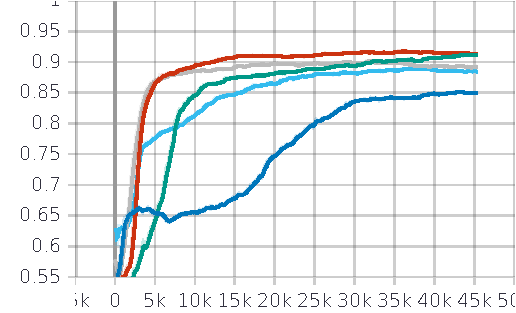
\includegraphics[width=0.45\textwidth]{img/exp11acc.pdf}}
    \subfigure[Wide experiment 2: accuracy]{
        \label{fig:exp12acc}
        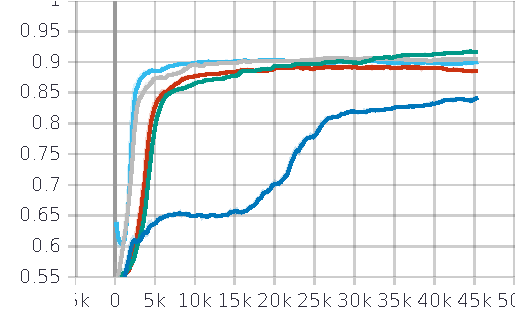
\includegraphics[width=0.45\textwidth]{img/exp12acc.pdf}}
    \subfigure[Wide experiment 1: loss]{
        \label{fig:exp11loss}
        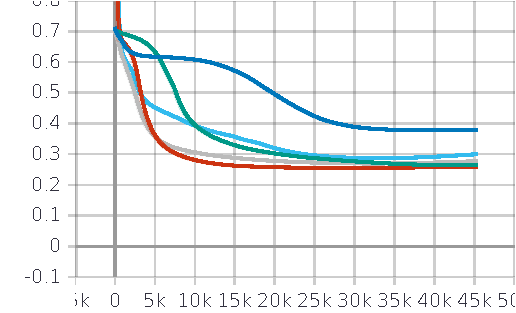
\includegraphics[width=0.45\textwidth]{img/exp11loss.pdf}}
    \subfigure[Wide experiment 2: loss]{
        \label{fig:exp12loss}
        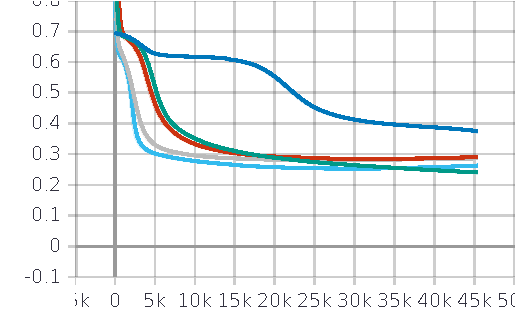
\includegraphics[width=0.45\textwidth]{img/exp12loss.pdf}}
    \subfigure[Legend]{
        \label{fig:legendexp1}
        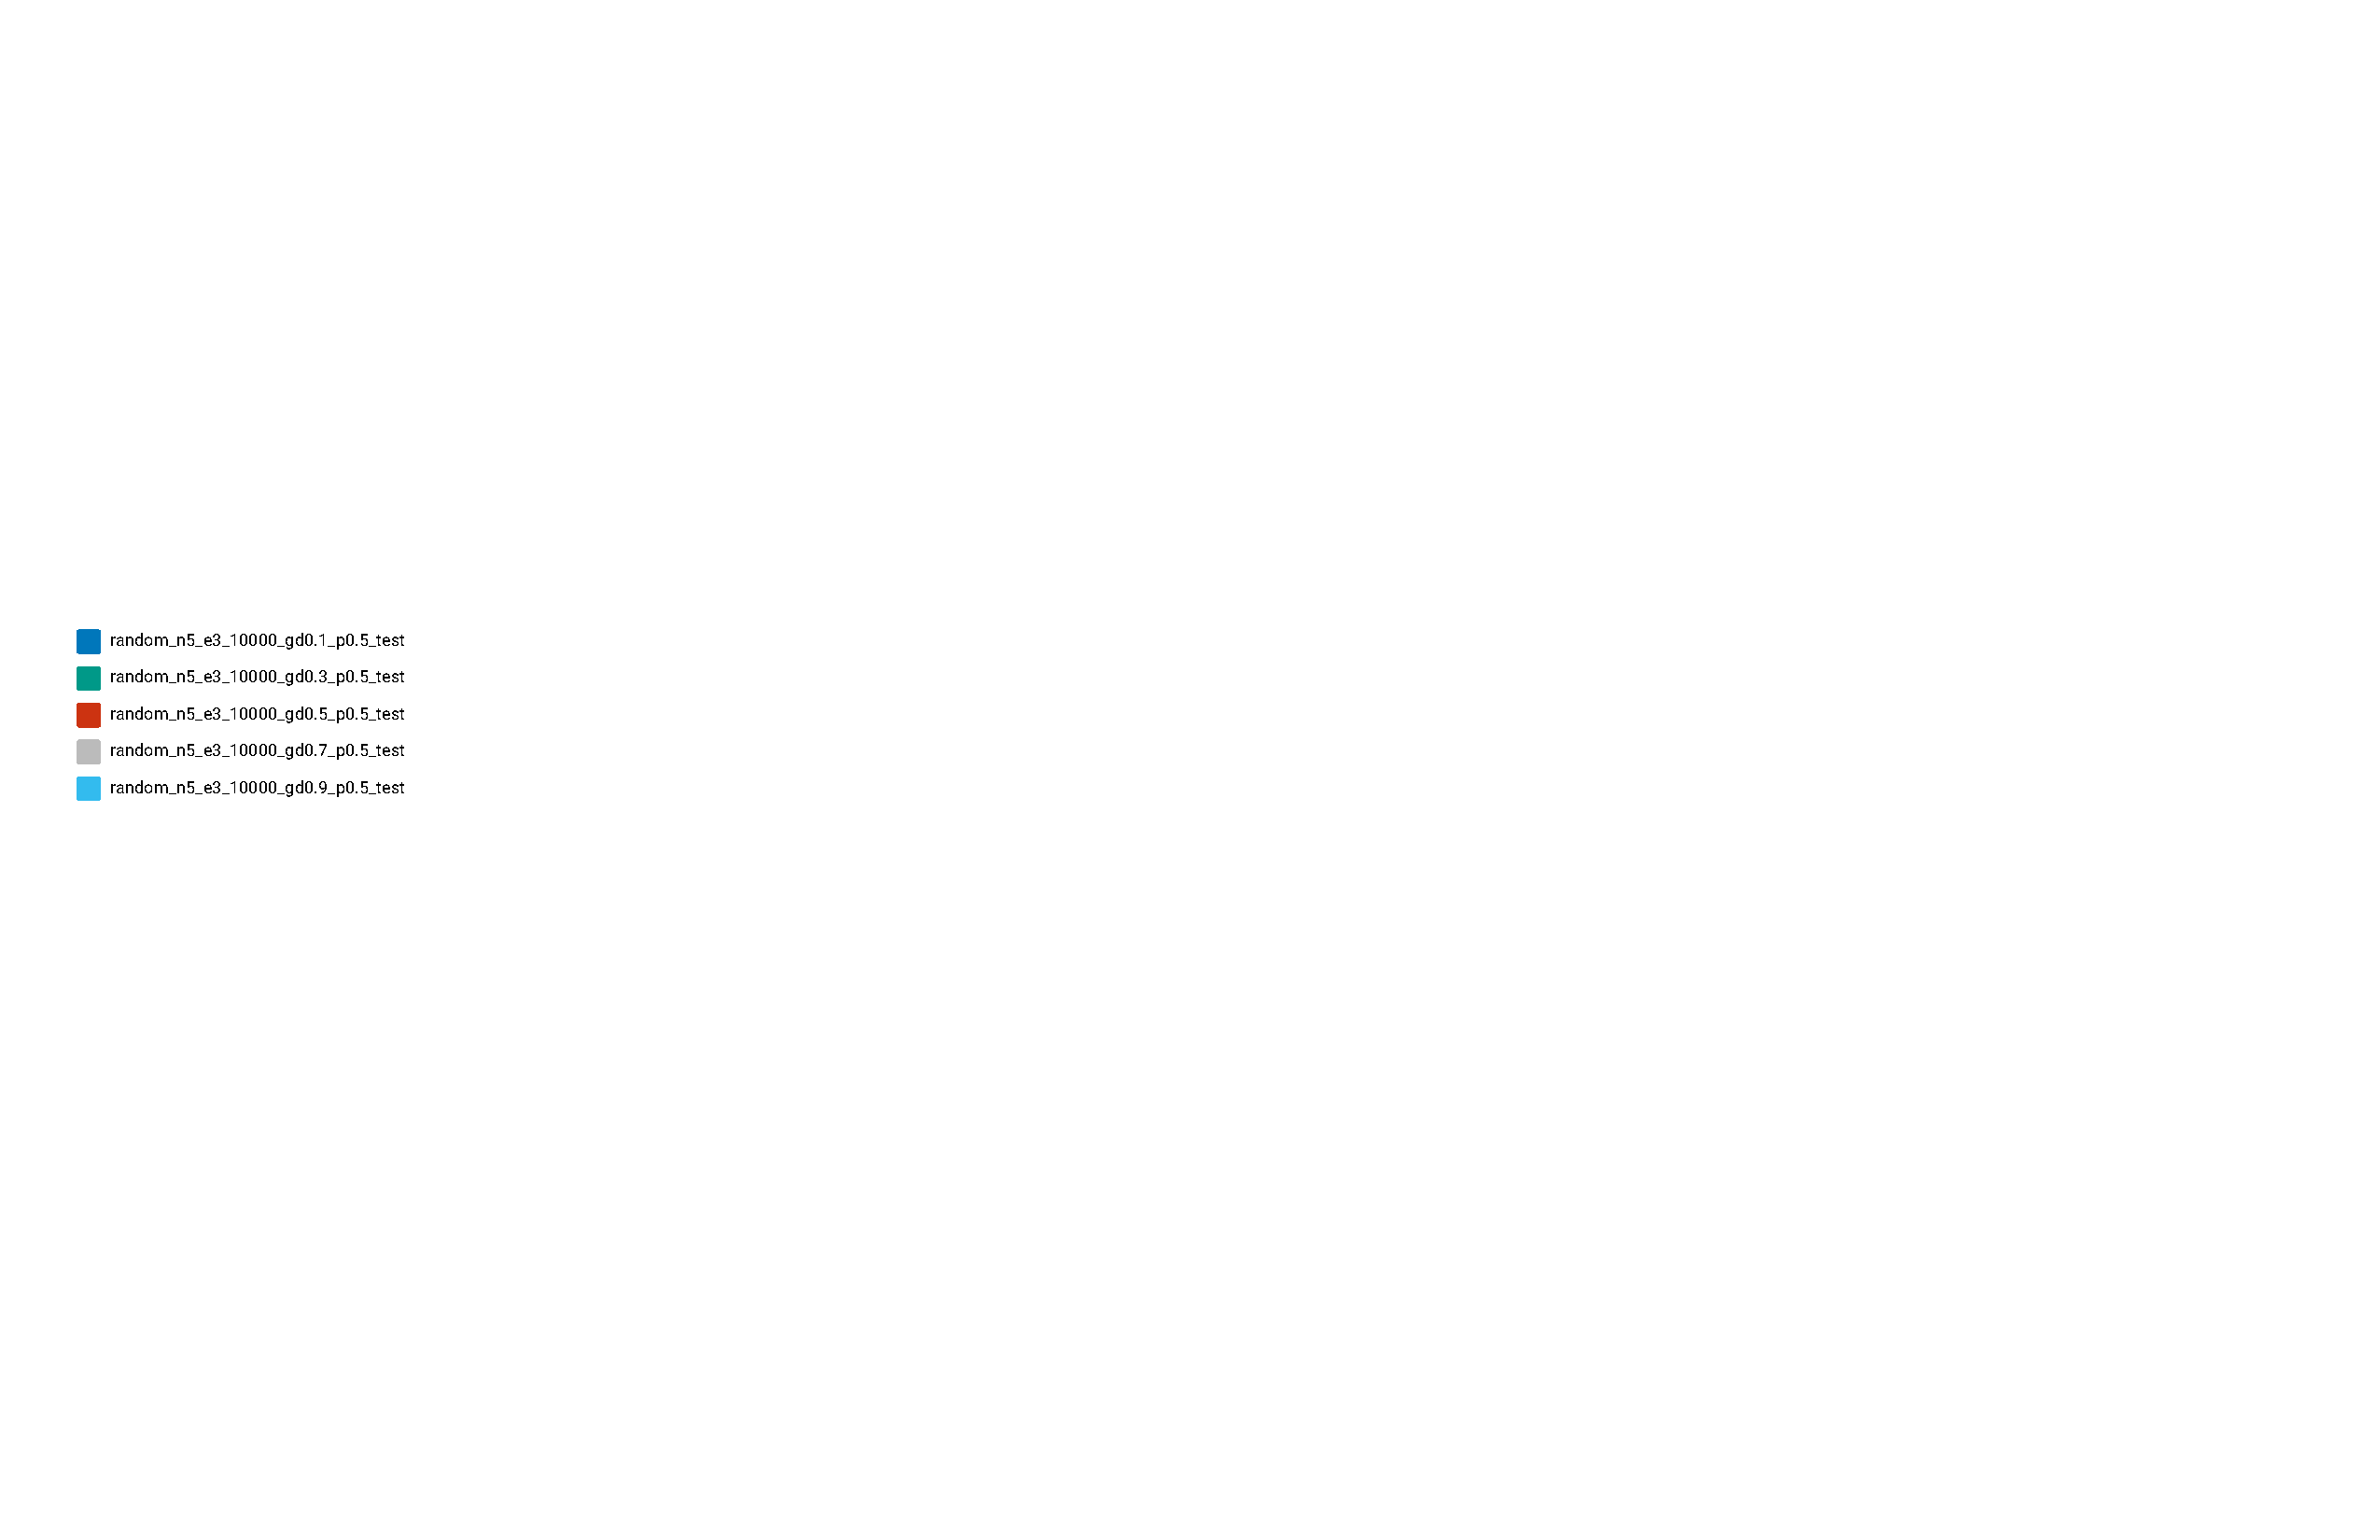
\includegraphics[width=0.4\textwidth]{img/legendexp1.pdf}}
    \caption{Result of wide experiment 1 and 2}
    \label{fig:resw12}
\end{figure}

The first conclusion is that this kind of neural network can learn the logical concept like bisimulation.
Most cases showed approximately 85\% accuracy when 500 epochs end.
This reveals the train is successful and the network actually catches the concepts of bisimulation.
Compare all training, the graphs with 0.1 as density (i.e. most sparse) are harder for the network to be trained.
Intuitively, the graphs with more link can express more complicated logic.
And should be harder for the network to learning the feature.
However, it may because the dense graph will show less complicate bisimulation propriety.
In other words, when the graph becomes denser, the bisimulation pattern may go more simple.
Concretely, for a dense graph, the mini bisimilar equivalent graph will most likely be either completely same (e.g. Figure \ref{fig:outputg3}) or be one node with self-loop of all possible link (e.g. Figure \ref{fig:outputg4}).
For the first situation, two bisimilar graphs will be isomorphic (i.e. nodes of two graph are connected in the same way, only the sequence of the nodes is different).
In this situation, the problem turns to distinguish if two graphs are isomorphic, which is much easier.
For the second situation, the graph can be represented in a graph with one node.
In this situation, the graphs are bisimilar may be diverse.
But graphs that are not bisimilar may have a big difference which will make the task easier.

The wide experiment can guide the deep experiment.
The result of wide experiment indicates that using random test case generator sample form the space of possible graphs is practicable (i.e. the performance of the algorithm when feeding dataset generated by one generator is representative).
Because, except the one training (i.e. generator has 0.1 as density), most training show similar results.
It reveals that the result of training for graphs with a certain scale can be represented by the training that bases on the data generated by a random test case generator.

\subsubsection*{Deep Experiment}
The purpose of the deep experiment is to test the capability of the neural network.
Thus in this experiment, graphs used here will be larger (i.e. has more nodes while maintaining the same number of edge type).
According to the learning curve and where the accuracy converges, the capability of this neural network can be estimated.

In this experiment, only the number of nodes for the generated graphs will change (see Listing \ref{lst:deepexp}). 
And the \texttt{graph\char`_density} will be 0.5.
Since in the wide experiment, the test cases generated with 0.5 graph density can better represent the overall leaning states (see Figure \ref{fig:resw12}).

\begin{figure}[h]
    \centering
    \subfigure[Deep experiment 1: accuracy]{
        \label{fig:exp21acc}
        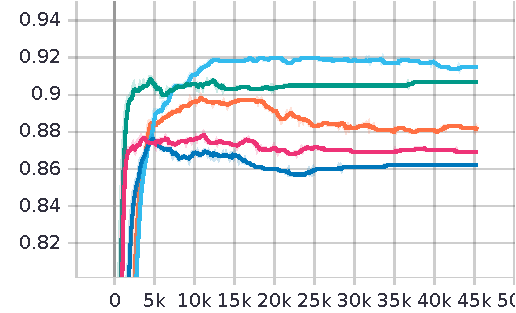
\includegraphics[width=0.45\textwidth]{img/exp21acc.pdf}}
    \subfigure[Deep experiment 2: accuracy]{
        \label{fig:exp22acc}
        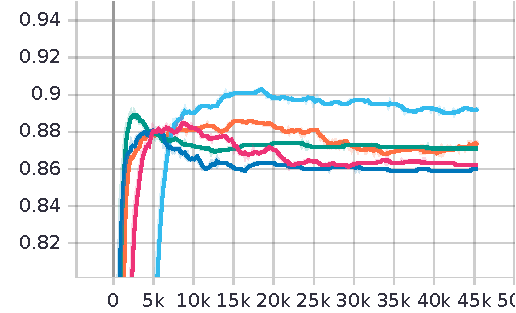
\includegraphics[width=0.45\textwidth]{img/exp22acc.pdf}}
    \subfigure[Deep experiment 1: loss]{
        \label{fig:exp21loss}
        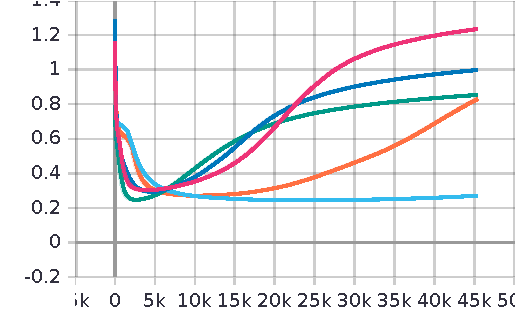
\includegraphics[width=0.45\textwidth]{img/exp21loss.pdf}}
    \subfigure[Deep experiment 2: loss]{
        \label{fig:exp22loss}
        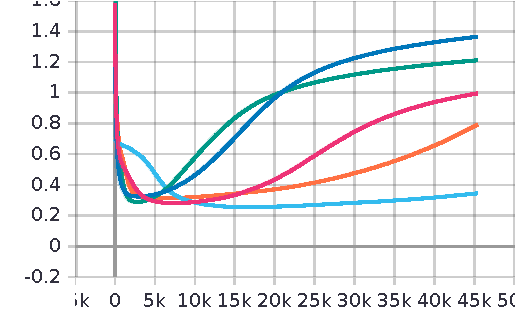
\includegraphics[width=0.45\textwidth]{img/exp22loss.pdf}}
    \subfigure[Legend]{
        \label{fig:legendexp2}
        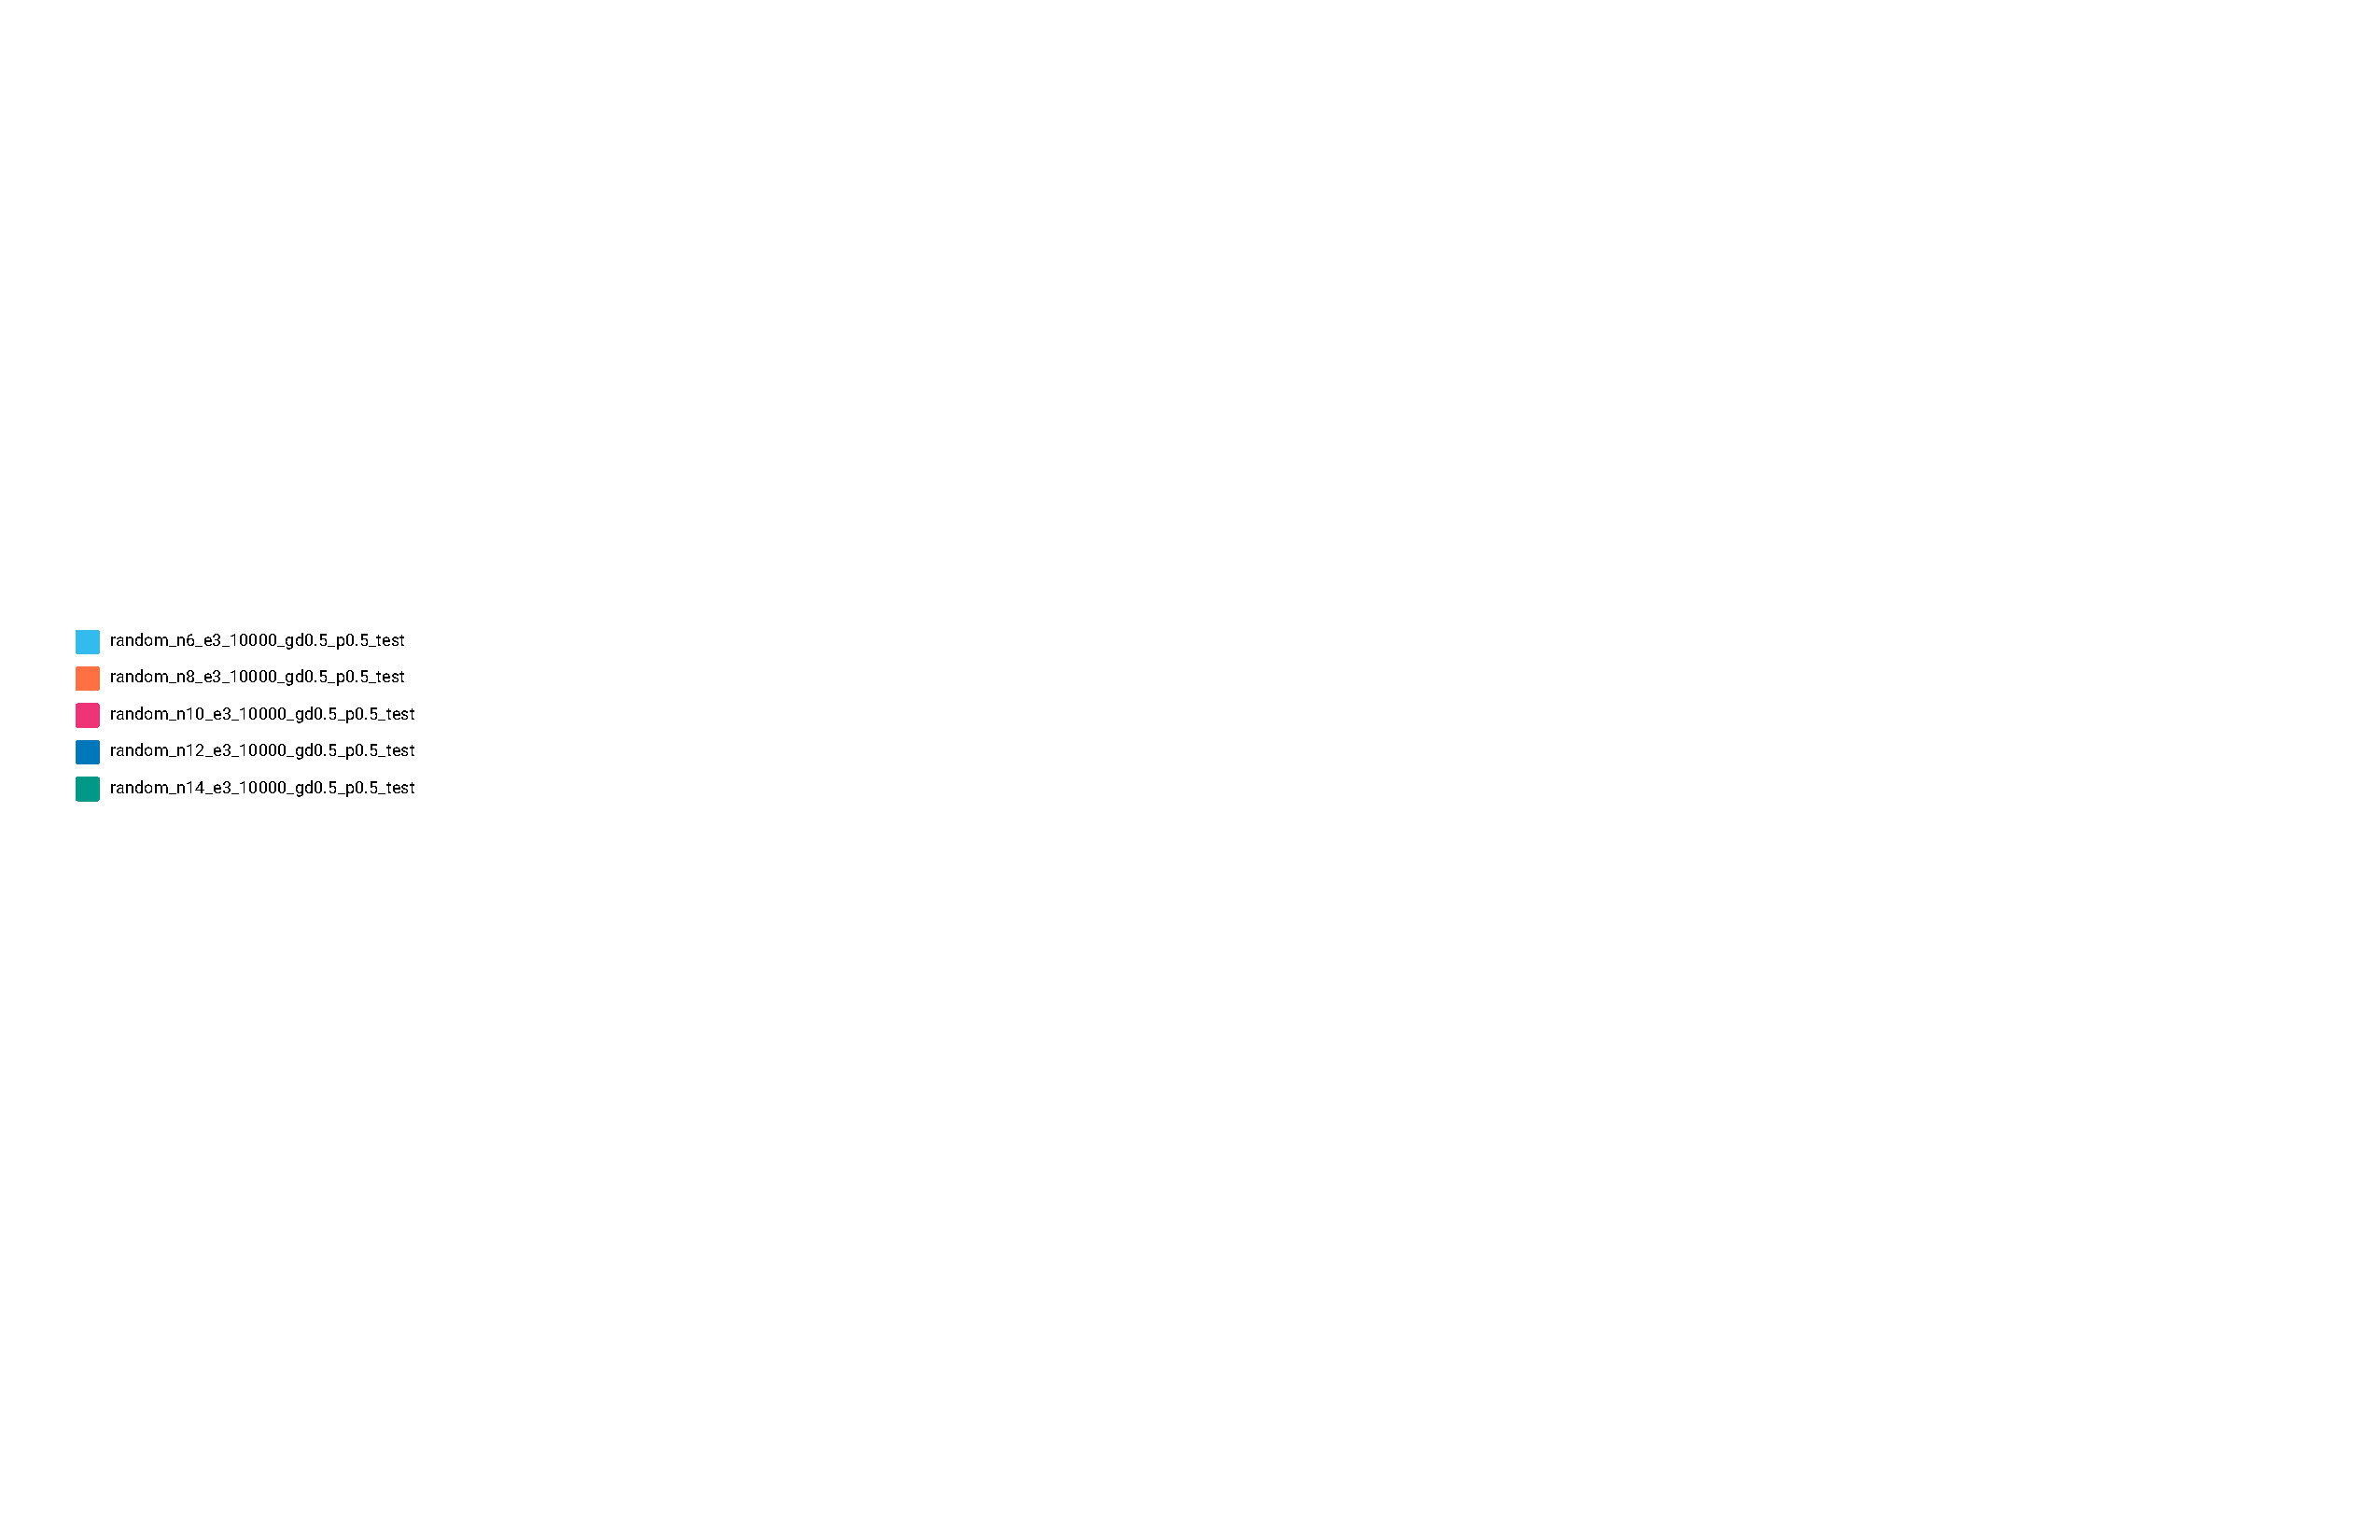
\includegraphics[width=0.4\textwidth]{img/legendexp2.pdf}}
    \caption{Result of deep experiment 1 and 2}
    \label{fig:resd12}
\end{figure}

The result is shown in Figure \ref{fig:resd12}.
Same as the wide experiment, in order to make graphs more clear, only the cases generated with \texttt{nodes\char`_num = 6, 8, 10, 12, 14} are shown in the graphs.
The model show the sign of overfitting, i.e. the learner start to learn very specific random features rather than the target feature.
Specifically, in the process of training, the loss of training set decreases while the loss on the test set is increasing.
Similarly, the accuracy becomes better on the training set, but worse on the test set.

While it also shows some interesting result which is unexpected.
For the aspect of training result, the value of accuracy will be compared.
Considering the overfitting, the accuracy will drop when training performed too much.
And for different training cases, the point of overfitting is different.
To reduce the effect of the overfitting, the peak of each line will be taken for comparison.
Form Table \ref{tab:pnl} and Figure \ref{fig:expdchart}, except for the case with 14 and 13 nodes, other cases show that accuracy is negatively correlated with the node number.
In other words, when the graphs are larger, it is harder for the network to infer bisimulation.
However, this correlation is not very significant. 
The differences between them are only around 10\%.
This may be caused by the small difference of the network.
Because, when facing different size of graphs, the input layer will increase the size in order to handle it.
It enhances the processing power of the network.
Yet there is still abnormality when it comes to the case of 13, 14 nodes.
This may be because of the quantity of the data.
Because the number of the possible graphs pairs explode from $2^150$ to $2^1176$.
And the quantity of the data is still 10000 groups.
Regarding the random generator as a sampling machine, for a much bigger space, the average difference of the two graphs took randomly will greater.
But the bisimilar pairs generated will be much similar.
Therefore, if the quantity of sampling is greater, the result may be more ``normal".
Since there will be more misleading cases.

From the training process, the graph with fewer nodes is hard to be learned.
The accuracy of the graph with least nodes (i.e. \texttt{random\char`_n6\char`_e3\char`_10000\char`_gd0.5\char`_p0.5\char`_test}) always converge slower than other cases.
But the accuracy of graph with most nodes (i.e. \texttt{random\char`_n14\char`_e3\char`_10000\char`_gd0.5\char`_p0.5\char`_test}) always increase fast than other.
Usually, the network with more nodes usually is considered more complicated.
And will need more time/epochs to learn.
However, in this case, the target learned is the bisimulation concept.
Much the same as the reason explained above, deficient of data may cause a big difference between negative and positive cases, which will lead to higher learning efficiency.

Generally speaking, the wide experiment proves that the performance of learning algorithm feeding with dataset generated by one random generator can be representative respect to the performance of all possible data space with the same scale.
In addition, the deep experiment did indicate that there may be a limitation of this neural network. 
However, there is still uncertainty exists.
Once the scale of graphs become bigger enough (i.e. bigger than 12) the situation becomes ``abnormal".
It may be coursed by the insufficient quantity of data.
And it still needs more experiments.


\begin{table}[h]
\centering
\small
\begin{tabular}{ |c|c|c| } 
 \hline
    \textbf{Nodes number} & \textbf{Accuracy experiment 1} & \textbf{Accuracy experiment 2} \\
 \hline
    5 & 0.917 & 0.888 \\
    6 & 0.920 & 0.902 \\
    7 & 0.900 & 0.865 \\
    8 & 0.898 & 0.885 \\
    9 & 0.883 & 0.889 \\
    10 & 0.878 & 0.884\\
    11 & 0.889 & 0.888\\
    12 & 0.874 & 0.880\\
    13 & 0.892 & 0.906 \\
    14 & 0.906 & 0.889 \\
 \hline
\end{tabular}
\caption{Peak accuracy of each line}
\label{tab:pnl}
\end{table}

\begin{figure}[h]
    \centering
    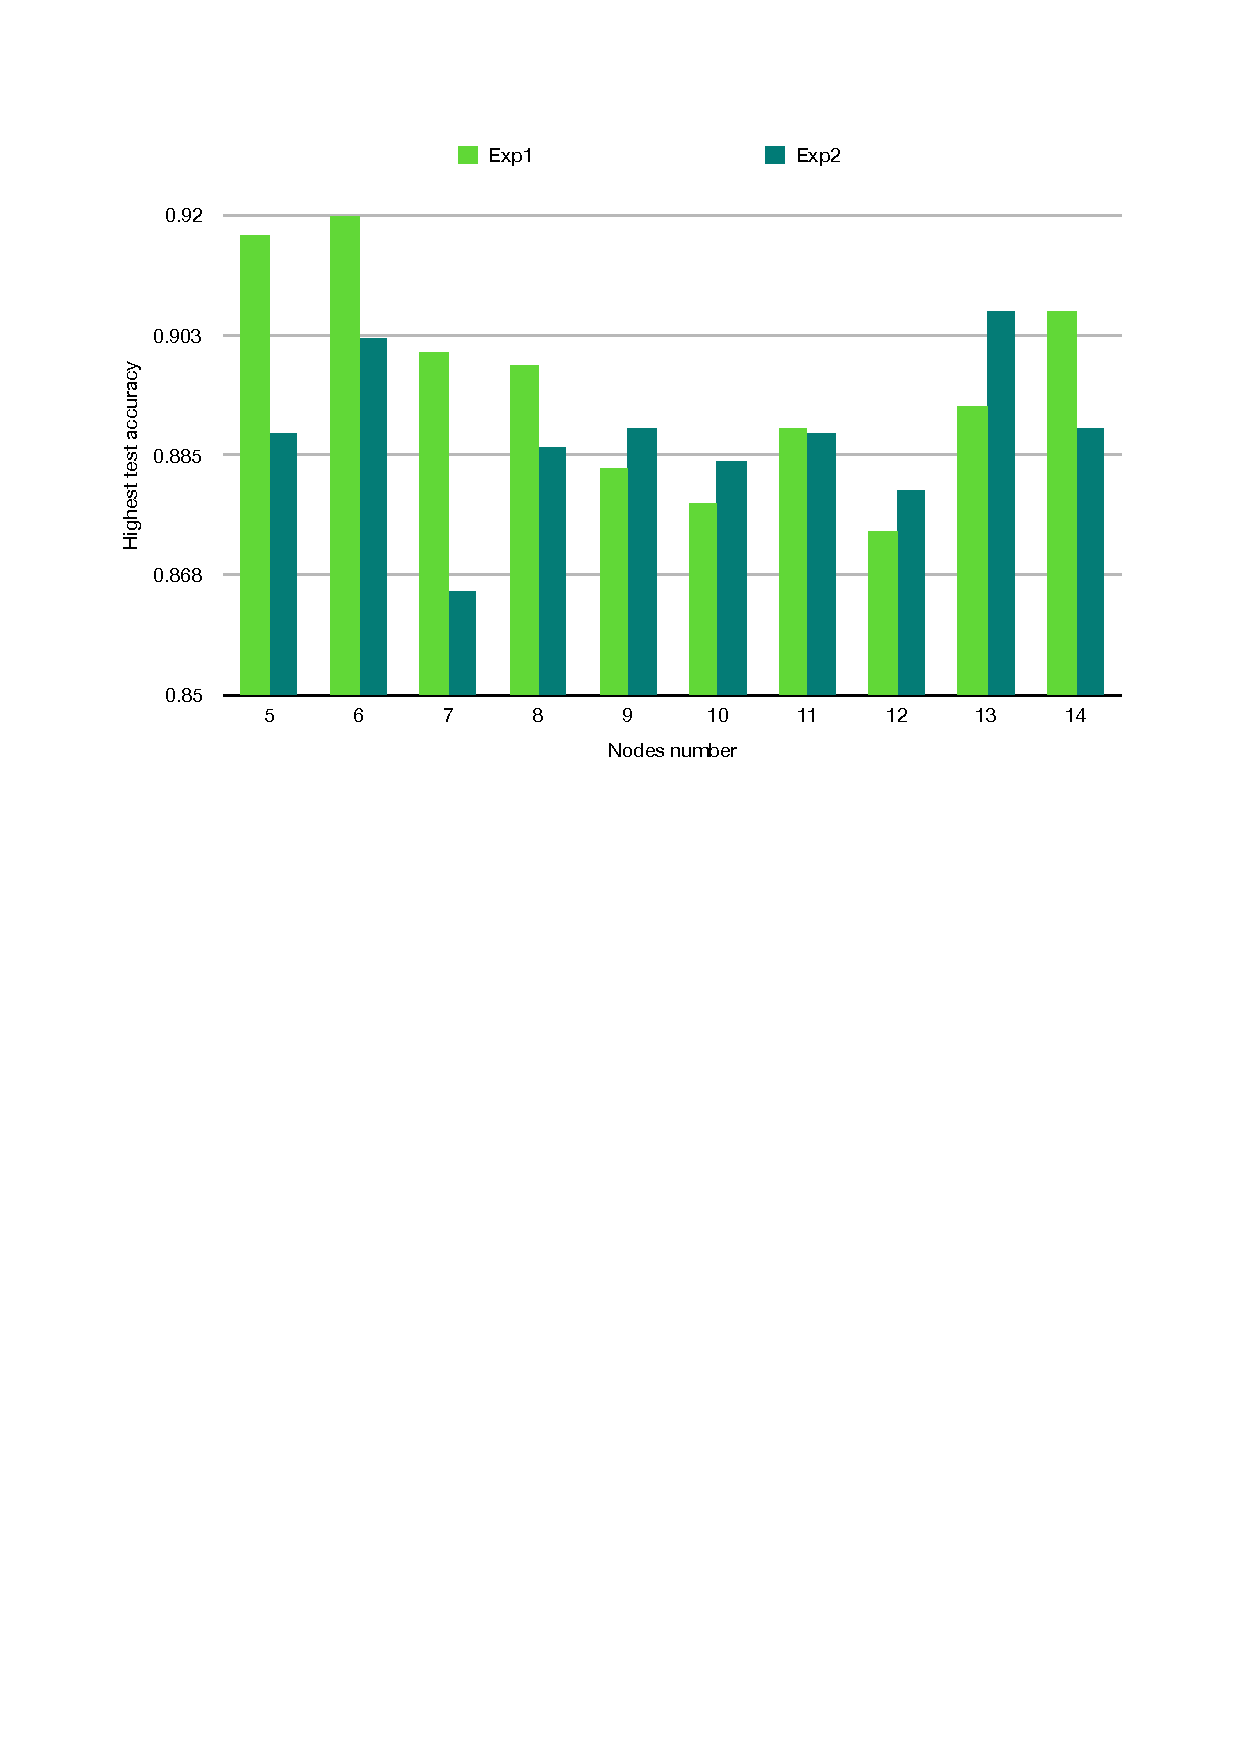
\includegraphics[width=\textwidth]{img/expdchart.pdf}
    \caption{Chart of test accuracy}
    \label{fig:expdchart}
\end{figure}




